\section{Proof Strategy}
For our proof, we show that, given a Coq model of both symbolic execution and the backwards symbolic execution tool and a set of properties, 
the backwards symbolic execution tool will give us a list of symbolic execution trees with corresponding leaves that, when executed, will result in an error state.

In other words, we define a list of symbolic execution trees, called \textit{tree\_list}, the we bind with a set of properties and a method to execute the relevant leaves, called \textit{execute\_tree\_list},
and show that it leads to a set of error states, called \textit{error\_states}. This can be expressed as the following theorem


\begin{theorem}
\label{thm:sufficiency}
$execute\_tree\_list (tree\_list) \in error\_states$.
\end{theorem}

The main structure of our proof is an inductive one. 
For our base case, we show that if the list only contains one tree, execution of that tree's root node with input specified by a selected leaf will result in an error state.

\begin{figure}
\label{fig:basecase}
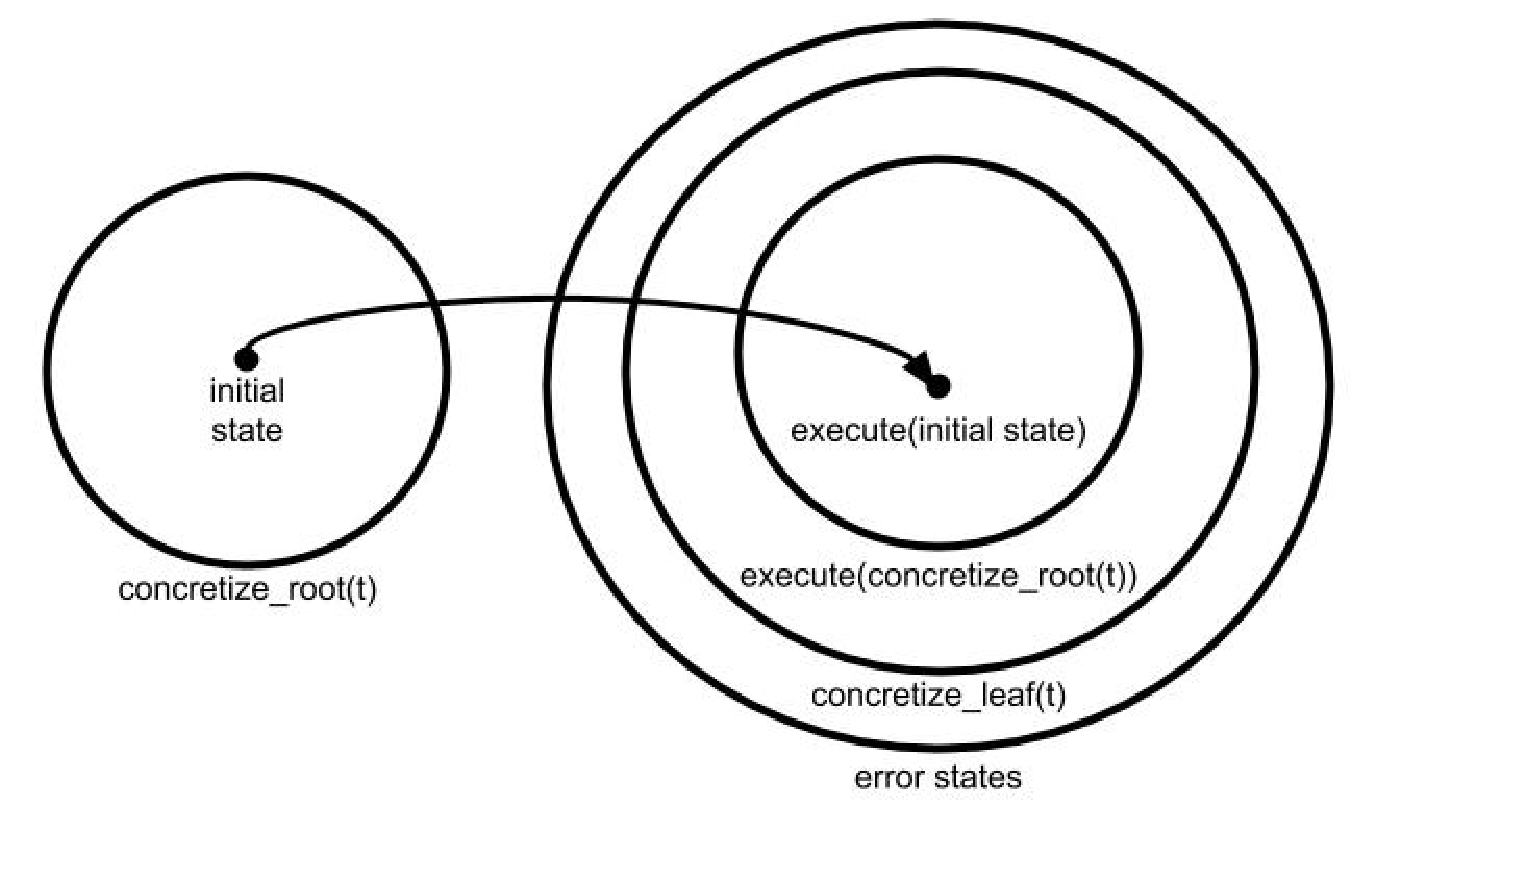
\includegraphics[width=\textwidth]{set3.eps}
\caption{Visual depiction of the base case of the proof.}
\end{figure}

In other words, as depicted in Figure \ref{fig:basecase}, we show that the initial state is an element of $concretize\_root(t)$ of the tree, $t$, and that concretely executing any element of $concretize\_root(t)$ will result n an element inside $concretize\_leaf(t).$
We then show that every element of $concretize\_leaf(t)$ is an error state, giving us our result.


For our inductive step, as depicted in Figures  \ref{fig:tlist} and \ref{fig:indstep}, we show that execution of each root with inputs from each specified leaf in a tree list of size $n$ will result in an error state using similar reasoning.

\begin{figure}
\label{fig:tlist}
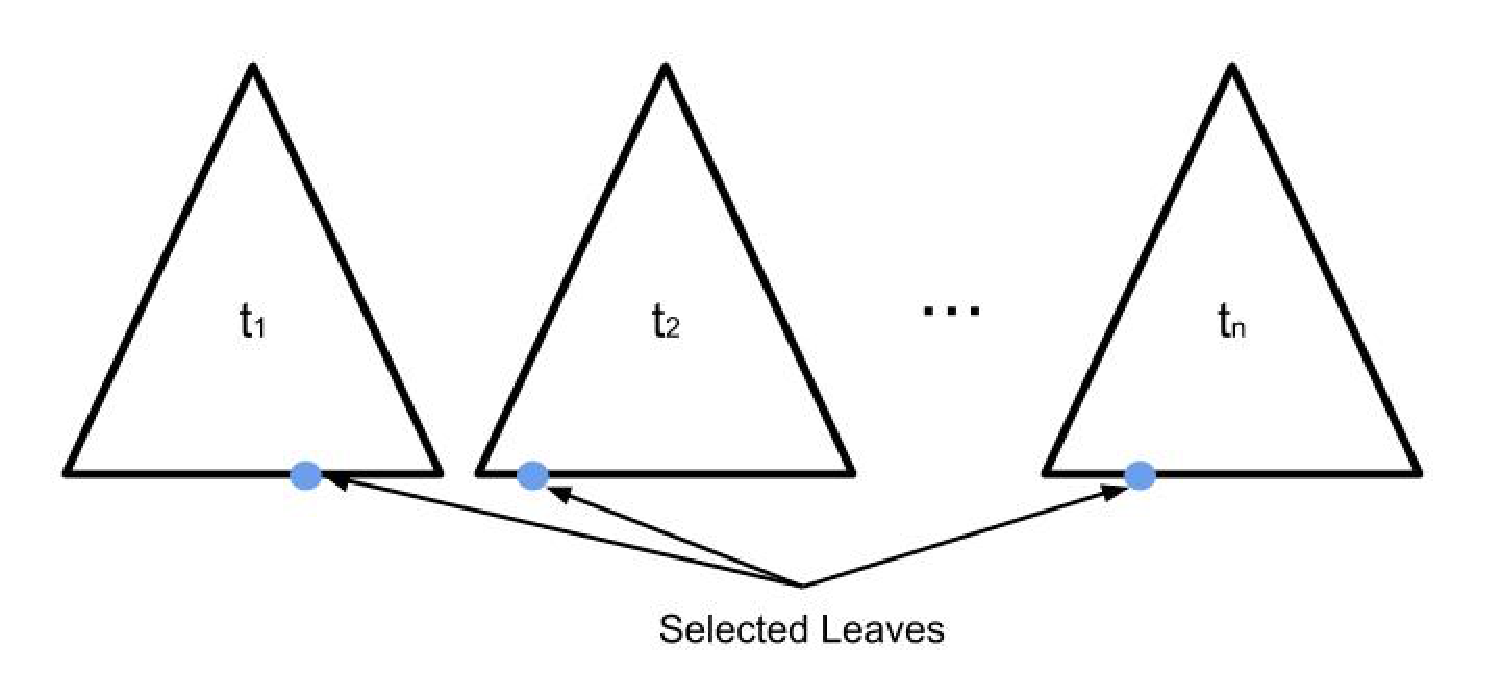
\includegraphics[width=\textwidth]{tlist.eps}
\caption{List of trees of length $n$.}
\end{figure}

\begin{figure}
\label{fig:indstep}
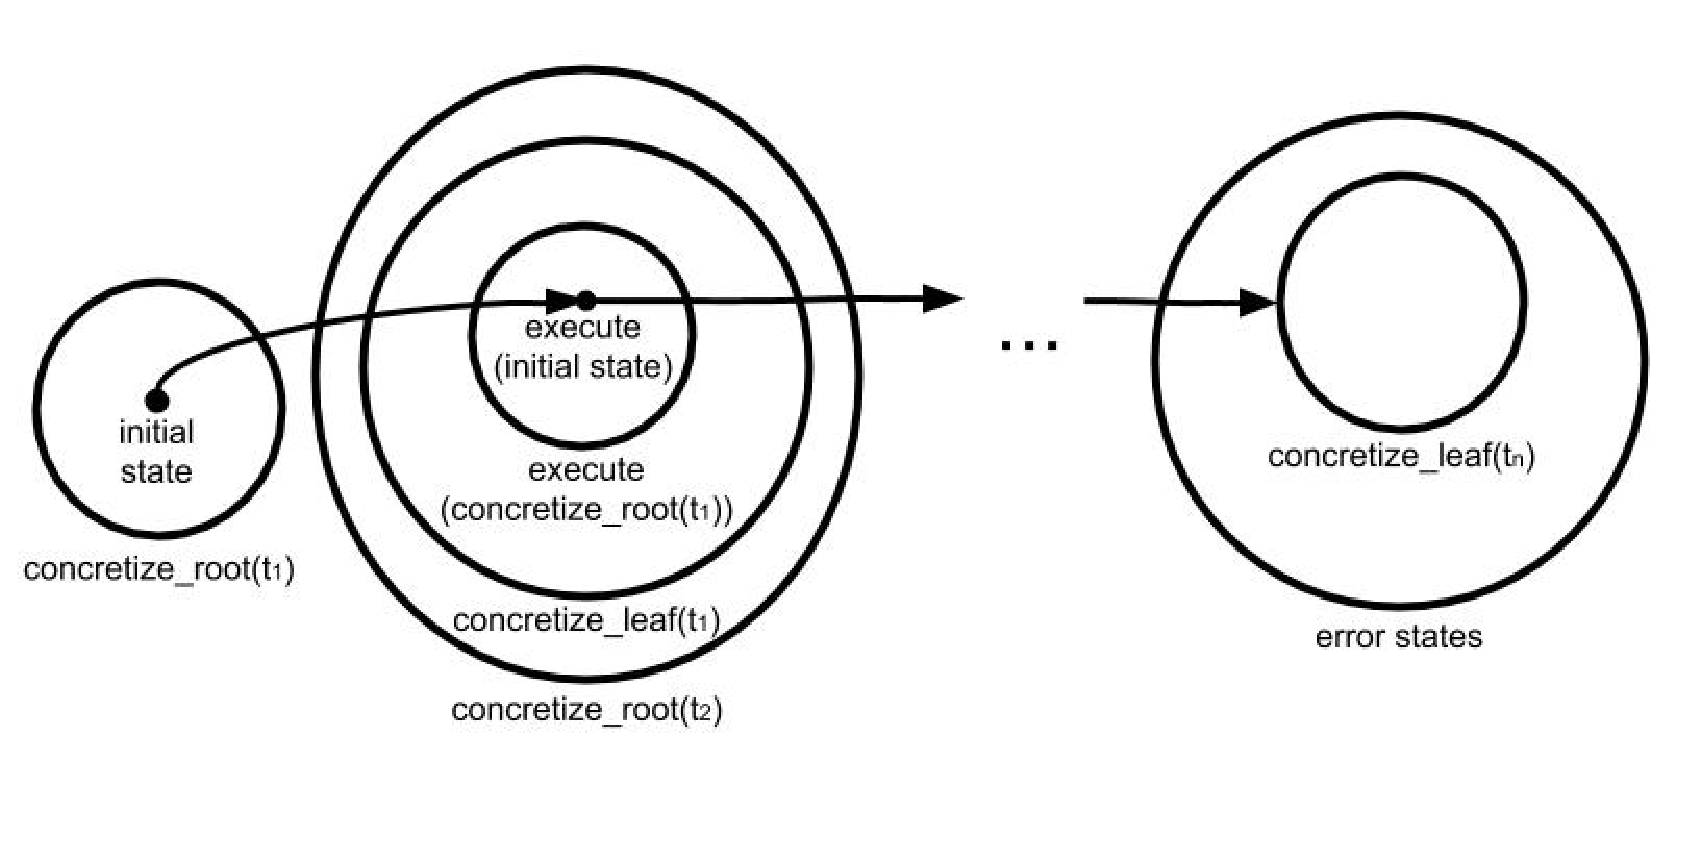
\includegraphics[width=\textwidth]{set4.eps}
\caption{Visual depiction of the inductive step of the proof.}
\end{figure}